%%    _____  _____
%%   |  __ \|  __ \    AUTHOR: Pedro Rivero
%%   | |__) | |__) |   ---------------------------------
%%   |  ___/|  _  /    DATE: November 10, 2021
%%   | |    | | \ \    ---------------------------------
%%   |_|    |_|  \_\   https://github.com/pedrorrivero
%%

%% ----------------------------------------------------------------------------

\begin{frame}{Introduction}

	Nature is described through the mathematical framework provided by \textbf{Quantum Field Theory}.

	\begin{multicols}{2}

		\begin{itemize}
			\item<2-> The different implementations of Quantum Field Theory are referred to as quantum field theories themselves.
			\item<3-> Quantum Chromodynamics (QCD) is the theory of the strong nuclear force.
			\item<3-> QCD holds many mysteries (e.g. \textbf{mass generation} phenomena).
			\item<4-> Many aspects of quantum field theories cannot be studied using classical computers.
      \item<4-> Physicists seek alternative tractable models to study interesting aspects of QCD.
		\end{itemize}

		\begin{center}
			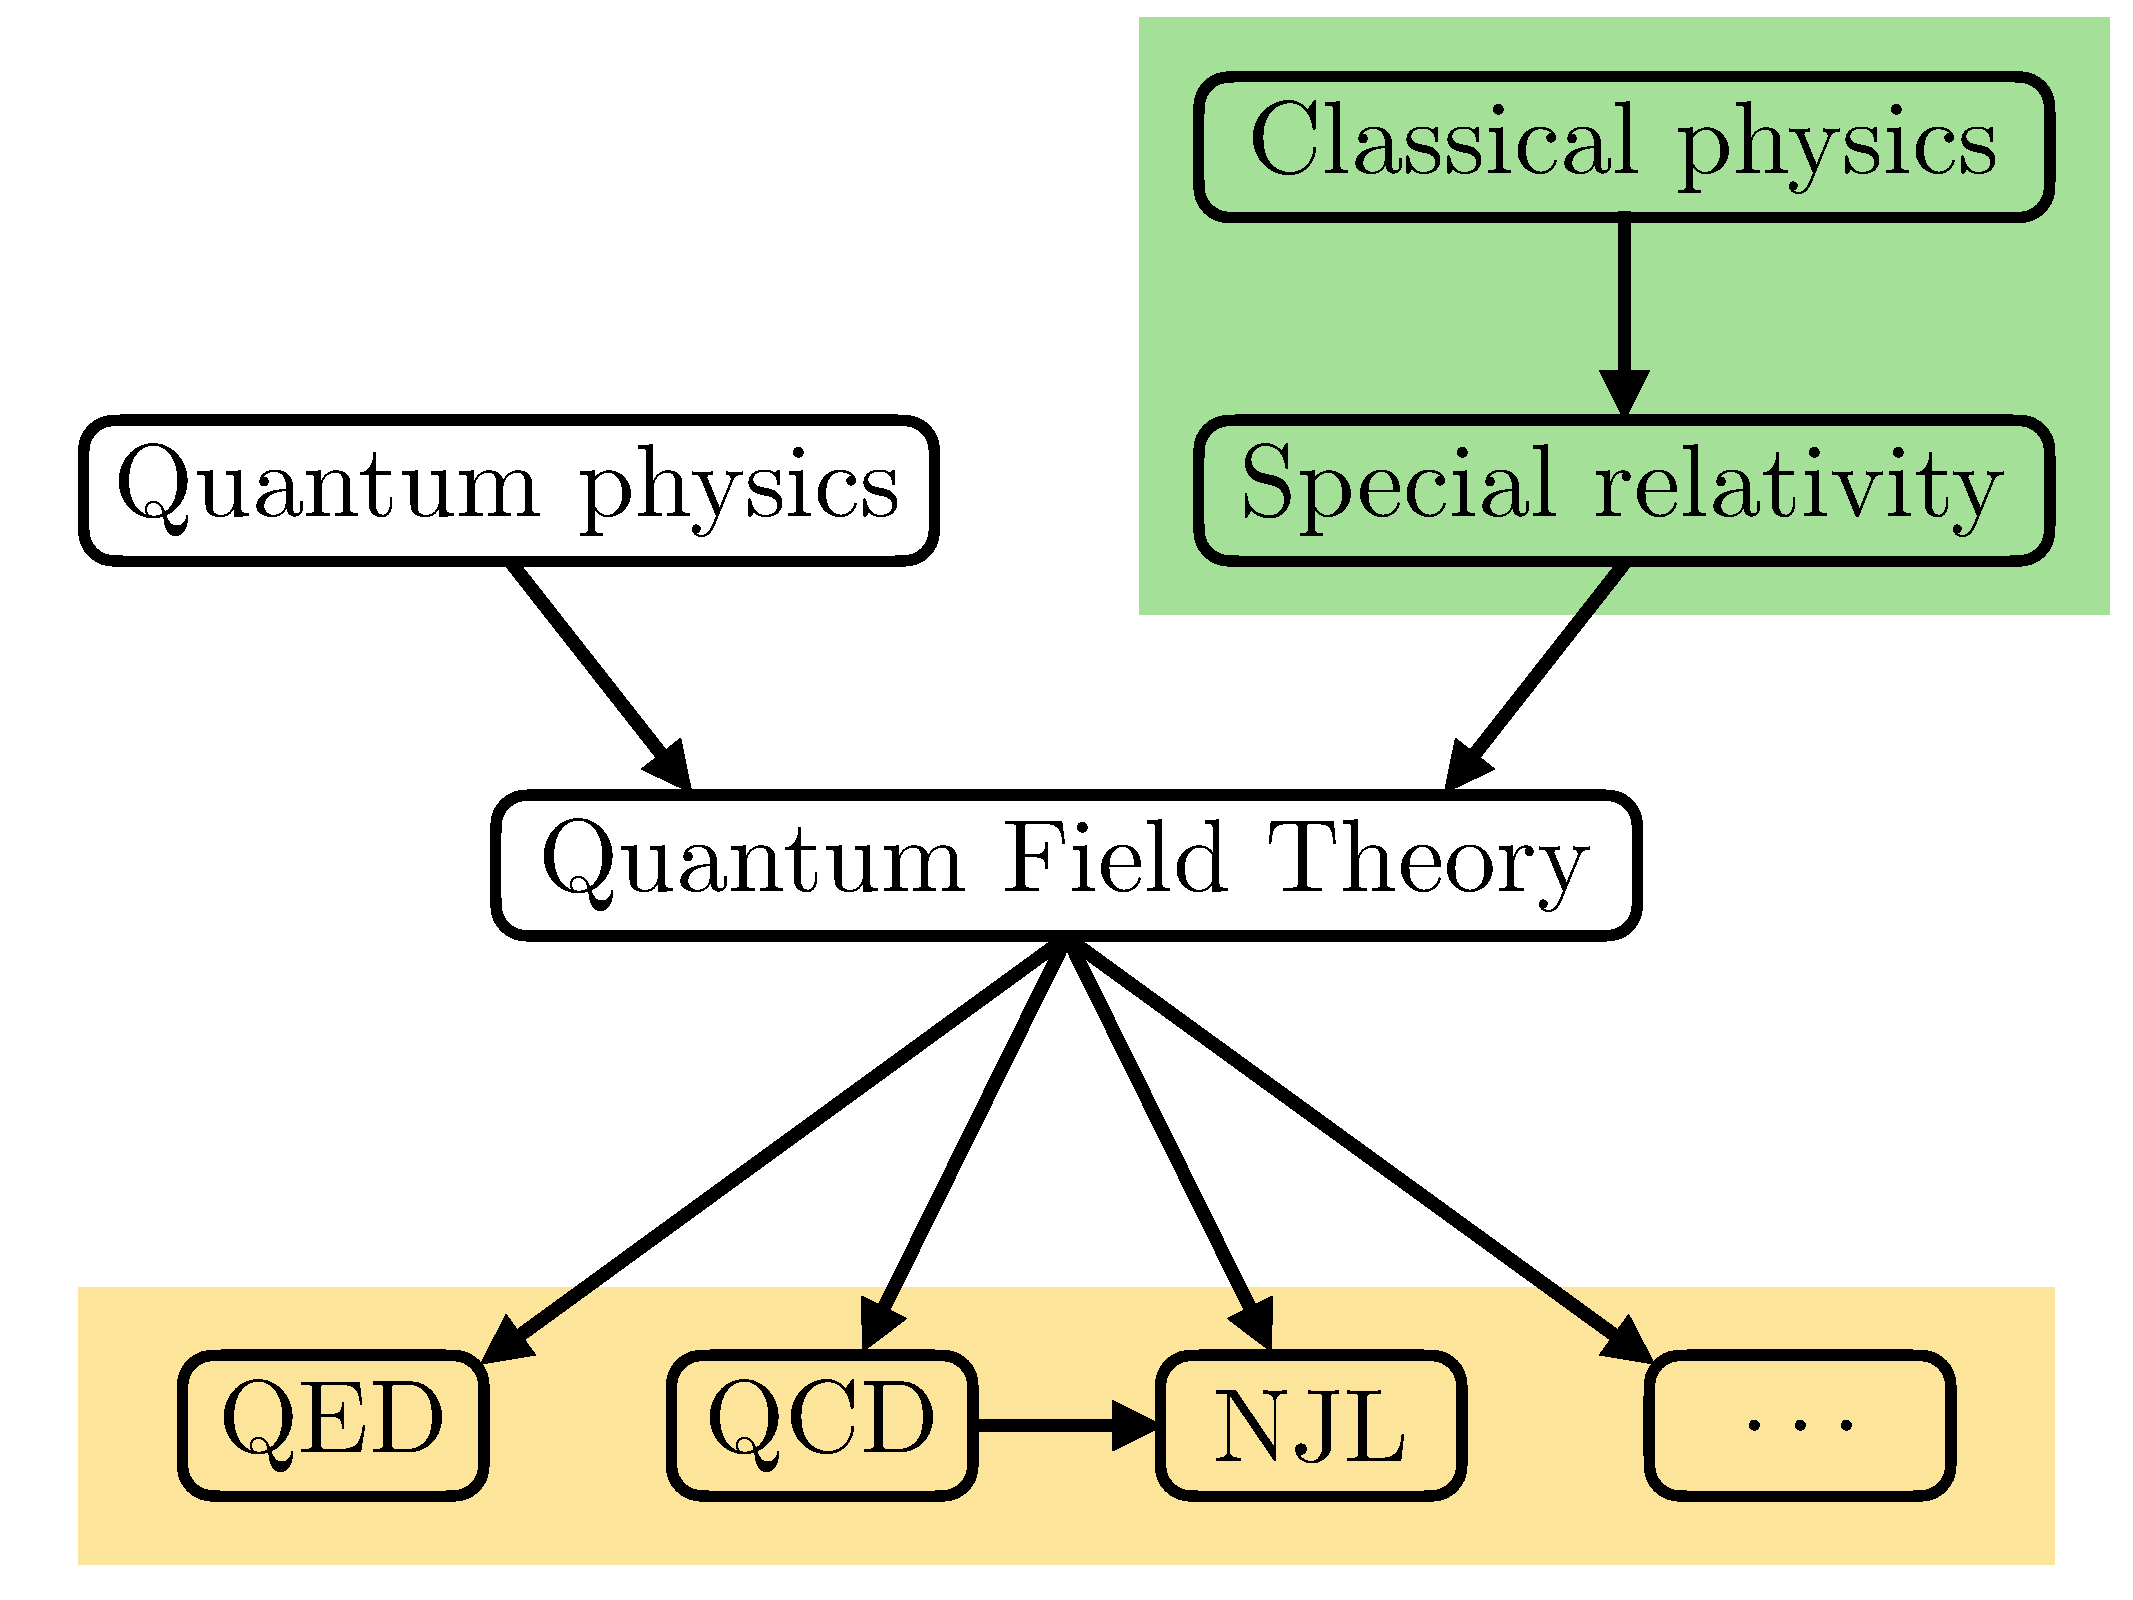
\includegraphics[width=.40\paperwidth]{Figures/quantum-field-theory}
		\end{center}

	\end{multicols}

\end{frame}

%% ----------------------------------------------------------------------------

% \begin{frame}{Objectives}
%
% 	An important path forward is to develop methods to simulate these models on quantum computers. This effort is only just beginning, however, performing calculations on a quantum computer is far from being a straightforward task; and it has only been achieved for relatively simple problems. My goal will be to develop some of the techniques necessary to use quantum computers for this endeavor. We will do so by analyzing the following:
%
% 	\medskip
%
% 	\begin{itemize}
% 		\item<2-> \textbf{Nambu--Jona-Lasino model} (NJL) in $1+1$ dimensions: an effective field theory, regarded as a low-energy approximation to QCD.
% 		\item<3-> It retains certain key features of QCD, such as the so called Goldstone modes and \textbf{dynamical chiral symmetry breaking}; which in turn is responsible for the creation of dressed mass.
% 		\item<4-> This model can be solved nonperturbatively through the standard leading order truncation; an important characteristic since verifying the solutions returned by any quantum computation is currently a major challenge.
% 	\end{itemize}
%
% \end{frame}
